\section{Zucchero sintattico}
\label{sec:2-syntactic-sugar}

Con lo scopo di rendere il codice più leggibile, conciso e semplice, \textbf{Funx} introduce
alcuni zuccheri sintattici (del tutto simili a quelli di \texttt{Haskell}).
Oltre all'indispensabile per non dover fare parsing dell'indentazione
e a quelli più comuni per l'arrichimento del lambda calcolo, sono riportati in Tabella \ref{tab:2-sugar}
anche tutti gli operatori simbolici supportati al momento (assieme alla notazione per indicarne l'associatività e precedenza).

\newpage

\begin{table}[H]
    \begin{center}
        \renewcommand{\arraystretch}{1.3}
        \begin{tabularx}{\textwidth}{|p{16em}|X|}
            \hline
            \textbf{Zucchero}                & \textbf{Sostituzione}                                            \\
            \hline
            \texttt{if b then e1 else e2 fi} & \texttt{if b then e1 else e2}                                    \\
            \hline
            \texttt{let}                     &                                                                  \\
            \texttt{f1 = e1}                 & \texttt{let f1 = e1 $\cdot$ f2 = e2 in e3}                       \\
            \texttt{f2 = e2}                 &                                                                  \\
            \texttt{in e3}                   &                                                                  \\
            \hline
            \texttt{f3 = e3}                 &                                                                  \\
            \texttt{with}                    &                                                                  \\
            \texttt{f1 = e1}                 & \texttt{f3 = let f1 = e1 $\cdot$ f2 = e2 in e3}                  \\
            \texttt{f2 = e2}                 &                                                                  \\
            \texttt{out}                     &                                                                  \\
            \hline
            \texttt{$\backslash$x -> e}      & \texttt{$\lambda$x $\mathord{.}$ e}                              \\
            \hline
            \texttt{$\backslash$x y -> e}    & \texttt{$\lambda$x $\mathord{.}$ $\lambda$y $\mathord{.}$ e}     \\
            \hline
            \texttt{f x y = e}               & \texttt{f = $\lambda$x $\mathord{.}$ $\lambda$y $\mathord{.}$ e} \\
            \hline
        \end{tabularx}
        \begin{tabularx}{\textwidth}{|p{8em}@{\quad}p{7em}|X|}
            \texttt{e1 $\mathord{.}$ e2} & \texttt{infixr 9} & \texttt{compose e1 e2}            \\
            \texttt{e1 / e2}             & \texttt{infixl 7} & \texttt{divide e1 e2}             \\
            \texttt{e1 \% e2}            & \texttt{infixl 7} & \texttt{modulo e1 e2}             \\
            \texttt{e1 * e2}             & \texttt{infixl 7} & \texttt{multiply e1 e2}           \\
            \texttt{e1 + e2}             & \texttt{infixl 6} & \texttt{add e1 e2}                \\
            \texttt{e1 - e2}             & \texttt{infixl 6} & \texttt{subtract e1 e2}           \\
            \texttt{e1 > e2}             & \texttt{infix 4}  & \texttt{greaterThan e1 e2}        \\
            \texttt{e1 >= e2}            & \texttt{infix 4}  & \texttt{greaterThanEquals e1 e2}  \\
            \texttt{e1 < e2}             & \texttt{infix 4}  & \texttt{lessThan e1 e2}           \\
            \texttt{e1 <= e2}            & \texttt{infix 4}  & \texttt{lessThanEquals e1 e2}     \\
            \texttt{e1 == e2}            & \texttt{infix 4}  & \texttt{equalsEquals e1 e2}       \\
            \texttt{e1 != e2}            & \texttt{infix 4}  & \texttt{notEquals e1 e2}          \\
            \texttt{!!e}                 & \texttt{prefix 4} & \texttt{not e}                    \\
            \texttt{e1 \&\& e2}          & \texttt{infixr 3} & \texttt{if e1 then e2 else False} \\
            \texttt{e1 || e2}            & \texttt{infixr 2} & \texttt{if e1 then True else e2}  \\
            \texttt{e1 \$ e2}            & \texttt{infixr 0} & \texttt{apply e1 e2}              \\
            \hline
        \end{tabularx}
    \end{center}
    \caption{Zuccheri sintattici}
    \label{tab:2-sugar}
\end{table}

\newpage

\noindent Come già accennato, il Capitolo \ref{chap:5-compiler} illustrerà come l'albero sintattico astratto (\texttt{AST})
di un programma viene ottenuto, annotato e tradotto in \texttt{Java}; la sezione \ref{sec:5-lazy-evaluation}
in particolare esporrà il motivo della traduzione degli operatori booleani binari in if.

\noindent Un esempio di programma e corrispondente \texttt{AST} sono presentati nel Codice \ref{lst:2-example} e Figura \ref{fig:2-example};
seppur superflua, l'indentazione è inclusa per maggiore chiarezza,
e le annotazioni di tipo sono state omesse poiché approfondite nel Capitolo \ref{chap:3-inference}.

\vspace{8mm}
\begin{lstlisting}[caption={Esempio di programma}, style=funxCode, label={lst:2-example}]
main = equalsEquals 499751156776108032 . multiply (tetration 3 3) . tetration 2 $ 4

tetration a n = if n == 0 then 1 else power a $ tetration a (n - 1) fi
    with
        power b e = if e == 0 then 1 else b * power b (e - 1) fi
    out
\end{lstlisting}

\begin{figure}[H]
    \centering
    \vspace{8mm}
    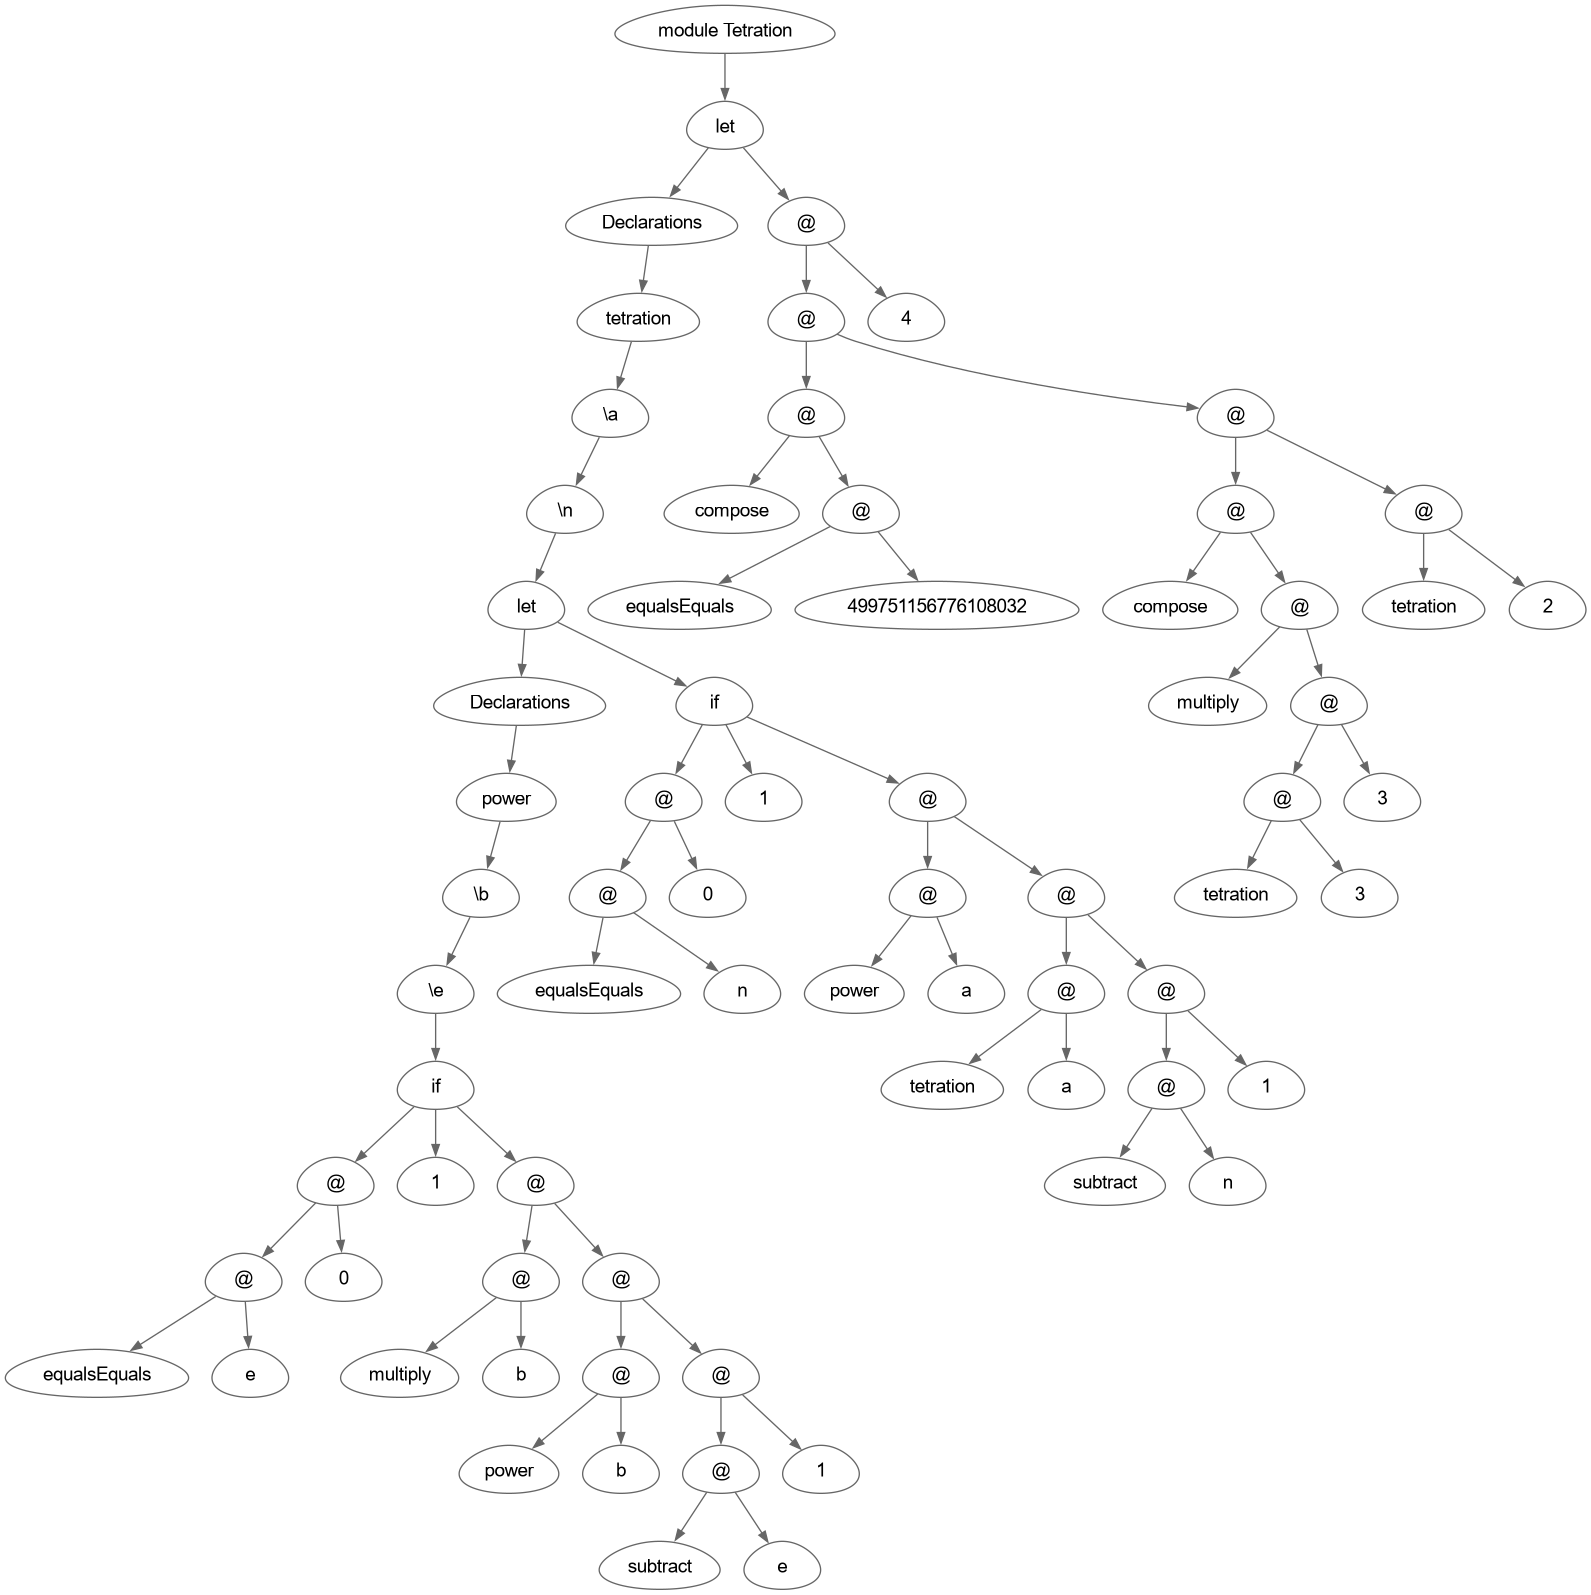
\includegraphics[width=\textwidth]{2-example}
    \caption{Esempio di AST}
    \label{fig:2-example}
\end{figure}